\label{DiagAlg}
\begin{center}
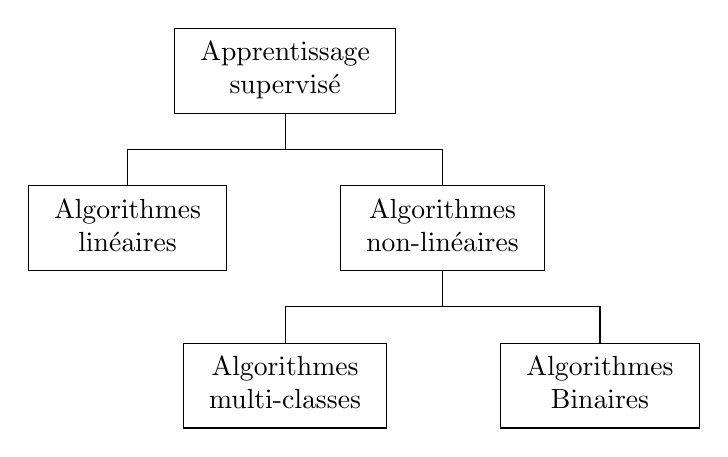
\begin{tikzpicture}
\begin{scope}
\node (AS) at (0,4.9) [rectangle,draw] {\begin{tabular}{c}Apprentissage\\ supervisé\end{tabular} };
\node (ASL) at (-2,2.9) [rectangle,draw] {\begin{tabular}{c}Algorithmes\\ linéaires\end{tabular} };
\node (ASNL) at (2,2.9) [rectangle,draw] {\begin{tabular}{c}Algorithmes\\ non-linéaires\end{tabular} };
\node (ASIM) at (0,0.9) [rectangle,draw] {\begin{tabular}{c}Algorithmes\\ multi-classes\end{tabular} };
\node (ASNM) at (4,0.9) [rectangle,draw] {\begin{tabular}{c}Algorithmes\\Binaires\end{tabular} };
\draw (AS) -- (0,3.9);
\draw (0,3.9) -| (ASNL);
\draw (0,3.9) -| (ASL);
\draw (ASNL) -- (2,1.9);
\draw (2,1.9) -| (ASIM);
\draw (2,1.9) -| (ASNM);
\end{scope}
\end{tikzpicture}
\captionof{figure}{Diagramme des différents algorithme de classification.}
\end{center}
